\documentclass[9pt,twocolumn]{extarticle}
\usepackage[a4paper,top=30mm,bottom=20mm,left=10mm,right=10mm,columnsep=12.7mm]{geometry}
\usepackage{kotex}
\usepackage{fontspec}
\setmainfont{Times New Roman}
\setmainhangulfont[AutoFakeSlant=0.2]{HCR Batang}
\setsansfont{Times New Roman}
\setsanshangulfont[AutoFakeSlant=0.2]{HCR Batang}
\usepackage{amsmath,amssymb,booktabs,graphicx,xcolor}
\usepackage[font=small,labelsep=space]{caption}
\usepackage{titlesec}
\usepackage[ruled,linesnumbered]{algorithm2e}
\usepackage{placeins}
\usepackage{tikz}
\usetikzlibrary{arrows.meta,positioning,fit,calc,shapes.multipart}
\usepackage[hidelinks]{hyperref}
\graphicspath{{./}{../}}
\setlength{\parindent}{1em}
\setlength{\parskip}{0pt}
\setlength{\emergencystretch}{1.5em}
\renewcommand{\baselinestretch}{1.00}
\renewcommand{\refname}{참고문헌}
\renewcommand{\figurename}{그림}
\renewcommand{\tablename}{표}
\titleformat{\section}{\bfseries\fontsize{10.5}{12}\selectfont}{\thesection.}{0.5em}{}
\titleformat{\subsection}{\bfseries\fontsize{9.5}{11}\selectfont}{\thesubsection}{0.5em}{}
\titlespacing*{\section}{0pt}{1.0ex plus .2ex}{0.5ex}
\titlespacing*{\subsection}{0pt}{0.8ex plus .2ex}{0.35ex}
\SetAlFnt{\normalsize}
\SetAlCapFnt{\normalsize}
\SetAlCapNameFnt{\normalsize\bfseries}
\SetNlSty{scriptsize}{}{}
\SetKwInput{KwIn}{Input}
\SetKwInput{KwOut}{Output}
\SetKwFor{ForEach}{for each}{do}{end}
\DontPrintSemicolon

\begin{document}
\twocolumn[
\begin{@twocolumnfalse}
\begin{center}
{\fontsize{16}{19}\selectfont\bfseries 관측 행동 페르소나와 가정 기반 Uplift를 결합한\\
전자상거래 쿠폰 정책 시뮬레이터\par}
\vspace{3mm}
{\fontsize{14}{17}\selectfont\bfseries An E-Commerce Coupon Policy Simulator Combining Observed\\
Behavioral Personas with Assumption-Based Uplift\par}
\end{center}
\vspace{4mm}
\begin{center}
{\bfseries 요\hspace{1em}약}
\end{center}
\vspace{-1mm}
{\fontsize{9}{11}\selectfont
전자상거래의 쿠폰 정책은 즉시 구매뿐 아니라 재방문, 반복 노출 및 이탈 상태를
변화시키므로 단일 시점 구매예측만으로 평가하기 어렵다. 실제 서비스의 장기 온라인
탐색은 쿠폰비용과 사용자 피로를 유발하며, 공개 로그에서는 동일 사용자의 처치 및
비처치 잠재결과를 동시에 관측할 수 없다. 이에 본 연구는 관측 행동과 비식별
개입가정을 분리한 정책 실험용 사용자 시뮬레이터를 제안한다. REES46 Cosmetics
Shop 로그에서 masked bidirectional-GRU로 48차원 사용자 표현을 학습하고, 행동
빈도와 세션 내 전이를 이용해 페르소나와 lifecycle을 구성하였다. 2차 상태특징을
사용하는 maximum-entropy 선택모형과 이산 세션 간격 모형을 결합한 무쿠폰
생성기의 행동비율 RMSE는 0.0540이었다. Tianchi O2O의 비무작위 쿠폰 수령 차이는
인과효과 대신 합성환경의 보정 모멘트로 사용하였다. 독립 합성 표본의 가중 14일
반응 모멘트는 $\Delta_{\mathrm{pop}}^*=12.62\%p$와
$\widehat\Delta_{\mathrm{pop}}=12.55\%p$로 대응하였다. 주 1회 쿠폰 환경에서
1,000명, 13주 학습 후 별도 5,000명, 52주를 평가한 결과 discrete SAC는 사용자당
20.90회의 쿠폰으로 순이익 30,893.46을 기록하였다. 결과는 단일 seed와 가정 기반
uplift에 조건부이며 실제 인과효과의 증거로 해석하지 않는다.
\par\vspace{1mm}
\noindent\textbf{주제어:} 사용자 시뮬레이션, 행동 페르소나, Maximum Entropy IRL,
Uplift Modeling, Contextual Bandit, 강화학습\par}
\vspace{4mm}
\end{@twocolumnfalse}
]

\section{서론}
쿠폰 정책은 구매뿐 아니라 재방문과 이탈을 바꾸지만 실제 사용자 대상 장기 탐색에는
비용과 피로가 따른다. 또한 행동 로그에는 처치 반사실이 없고 비무작위 쿠폰 수령 차이는
선택편향을 포함한다. 이에 관측 행동과 가정 기반 개입효과를 분리한 정책 실험용
시뮬레이터를 제안한다.

행동 토큰을 복원하는 양방향 GRU로 사용자 표현을 학습하고, persona 조건부
maximum-entropy 선택모형과 세션 간격 모형으로 무처치 행동을 생성한다. Tianchi의
관측 차이는 canonical type과 쿠폰 감쇠항의 보정 모멘트로만 사용하며, 합성환경에서
bandit과 deep RL의 학습비용 및 장기 순이익을 비교한다.

순차 추천~\cite{sun2019}과 uplift modeling~\cite{devriendt2018}은 각각 행동 예측과
단일 결과의 증분 반응에 초점을 둔다. RecSim~\cite{ie2019}, RecoGym~\cite{rohde2018},
Virtual-Taobao~\cite{shi2019}와 달리 본 연구는 공개 데이터의 행동 생성과 쿠폰 반응을
분리하며, 쿠폰 모듈 제거 시 무처치 생성기로 환원된다.

\section{데이터}
주 행동 데이터는 REES46 Cosmetics Shop의 2019년 10월부터 2020년 2월까지 5개
CSV, 총 20,692,840행이다~\cite{rees46}. \texttt{user\_id mod 100=0}인 고정 약
1\% 표본 216,093행에서 최대 12,000명의 사용자 시퀀스를 구성하였다. 이벤트는
\texttt{view}, \texttt{cart}, \texttt{remove\_from\_cart}, \texttt{purchase}이며
명시적인 세션 ID를 제공한다. Electronics는 제거 행동이 없어 보조 분석에만 사용하였다.

쿠폰 반응 참고 자료는 Tianchi O2O 로그다~\cite{tianchi}. 2016년 5월 15일을 기준일로
두고, 기준일 수령 기록과 이후 14일 구매 기록을 비교하였다. 대리군은 기준일 이전
14일의 클릭과 구매만으로 정의하였다. 다섯 기준일의 placebo 구매율 차이가
6.85--8.87\%p이고 수령군의 후속 쿠폰 수령률도 12.11--31.31\%p 높아, 관측 차이를
인과적 CATE로 사용하지 않았다.

\section{제안 방법}
\subsection{Masked bidirectional-GRU 표현}
각 사용자의 행동 사이에 세션 경계 토큰을 삽입하고 앞 64개 토큰을 유지한다. 전체
유효 위치의 15\%를 마스킹하고 원래 토큰을 복원하도록 학습한다. 목적함수는
\begin{equation}
\mathcal{L}_{\mathrm{mask}}
=-\sum_{i\in\mathcal{M}}\log p_\psi(x_i\mid x_{\setminus\mathcal{M}})
\end{equation}
이다. 토큰 임베딩은 16차원, 양방향 GRU의 방향별 hidden size는 24이며, 양방향
마지막 상태를 연결한 48차원 벡터를 사용자 표현으로 사용한다. 실제 구현의 학습 및
표현 추출 과정은 알고리즘~\ref{alg:gru} 및 그림~\ref{fig:gru}에 제시한다.

\begin{algorithm}[!h]
\caption{Masked GRU embedding extraction}
\label{alg:gru}
\KwIn{$D=\{x_u\}$, masking rate $q$}
\KwOut{$Z=\{z_u\}$}
\ForEach{$B\subset D$}{
  $\widetilde B\leftarrow\operatorname{Mask}(B,q)$\;
  $H_B\leftarrow\operatorname{BiGRU}(E(\widetilde B))$\;
  $\psi\leftarrow\arg\min_\psi\mathcal L_{\mathrm{mask}}(B,H_B)$\;
}
$z_u\leftarrow\operatorname{Std}([\overrightarrow h_u;\overleftarrow h_u])$\;
\end{algorithm}

\subsection{행동 페르소나}
마스킹 GRU에서 얻은 48차원 사용자 임베딩에 $K=4$ K-means를 적용하여 P0--P3
집단을 구성하였다. 각 집단의 전체 관측 이벤트를 분모로 한 상대 이벤트 빈도는
그림~\ref{fig:eventmix}에 제시한다.

\begin{figure*}[!t]
\centering
\resizebox{0.90\textwidth}{!}{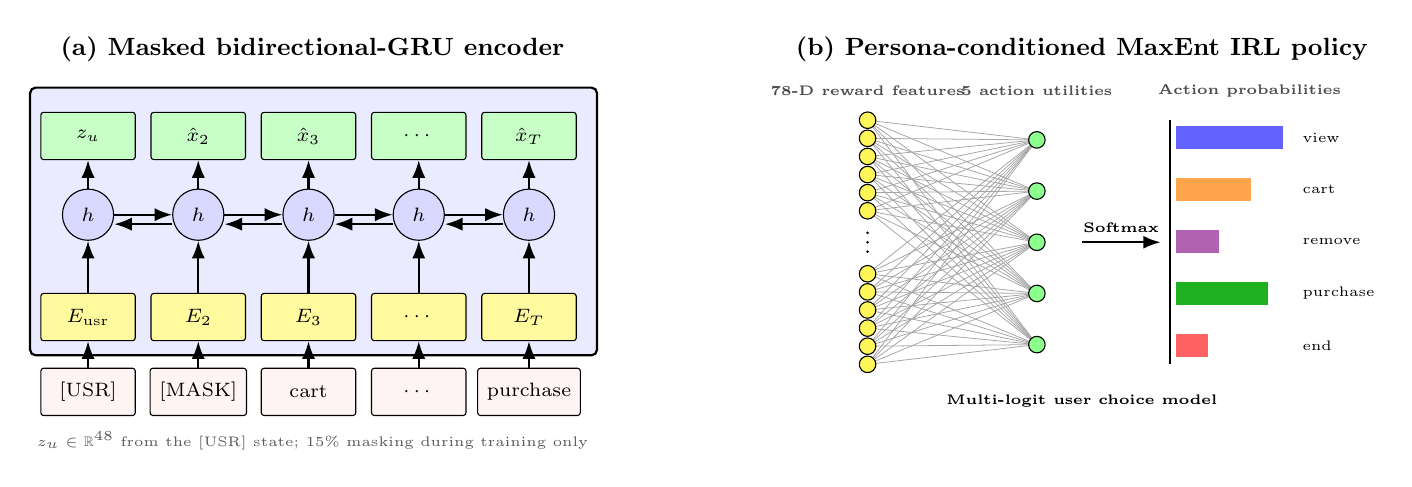
\begin{tikzpicture}[
  font=\scriptsize,
  >=Latex,
  arrow/.style={->, line width=0.75pt},
  token/.style={draw=black, rounded corners=1pt, minimum width=12mm,
                minimum height=6mm, align=center, fill=pink!18},
  embed/.style={draw=black, rounded corners=1pt, minimum width=12mm,
                minimum height=6mm, align=center, fill=yellow!38},
  state/.style={draw=black, circle, minimum size=6.5mm, fill=blue!15,
                inner sep=0pt},
  output/.style={draw=black, rounded corners=1pt, minimum width=12mm,
                minimum height=6mm, align=center, fill=green!22},
  side/.style={draw=black, rounded corners=1.5pt, minimum width=22mm,
               minimum height=7mm, align=center, fill=green!18},
  panel/.style={draw=black, rounded corners=2pt, fill=blue!8,
                line width=0.8pt},
  paneltitle/.style={font=\bfseries\small, align=center},
  layerlabel/.style={font=\scriptsize\bfseries, text=black!75}
]

% (a) Compact encoder architecture in the visual grammar of the BERT schematic.
\begin{scope}[xshift=0cm]
  \node[paneltitle] at (3.7,4.55) {(a) Masked bidirectional-GRU encoder};
  \node[panel, minimum width=72mm, minimum height=34mm, anchor=south west]
    (encbox) at (0.1,0.65) {};
  \foreach \x/\id/\tok/\emb/\out in {
    0.85/a/[USR]/$E_{\rm usr}$/$z_u$,
    2.25/b/[MASK]/$E_2$/$\hat{x}_2$,
    3.65/c/cart/$E_3$/$\hat{x}_3$,
    5.05/d/$\cdots$/$\cdots$/$\cdots$,
    6.45/e/purchase/$E_T$/$\hat{x}_T$} {
    \node[token] (tok\id) at (\x,0.20) {\tok};
    \node[embed] (emb\id) at (\x,1.15) {\emb};
    \node[state] (hid\id) at (\x,2.45) {$h$};
    \node[output] (out\id) at (\x,3.45) {\out};
    \draw[arrow] (tok\id) -- (emb\id);
    \draw[arrow] (emb\id) -- (hid\id);
    \draw[arrow] (hid\id) -- (out\id);
  }

  \draw[arrow] (hida) -- (hidb);
  \draw[arrow] (hidb) -- (hidc);
  \draw[arrow] (hidc) -- (hidd);
  \draw[arrow] (hidd) -- (hide);
  \draw[arrow] ([yshift=-1.2mm]hide.west) -- ([yshift=-1.2mm]hidd.east);
  \draw[arrow] ([yshift=-1.2mm]hidd.west) -- ([yshift=-1.2mm]hidc.east);
  \draw[arrow] ([yshift=-1.2mm]hidc.west) -- ([yshift=-1.2mm]hidb.east);
  \draw[arrow] ([yshift=-1.2mm]hidb.west) -- ([yshift=-1.2mm]hida.east);

  \node[font=\tiny, text=black!65, align=center] at (3.7,-0.42)
    {$z_u\in\mathbb{R}^{48}$ from the [USR] state; 15\% masking during training only};
\end{scope}

% (b) The 78-dimensional quadratic reward map converges to five utilities.
\begin{scope}[xshift=9.75cm]
  \node[paneltitle] at (3.72,4.55) {(b) Persona-conditioned MaxEnt IRL policy};
  \node[font=\tiny\bfseries, text=black!70] at (1.00,4.02)
    {78-D reward features};
  \node[font=\tiny\bfseries, text=black!70] at (3.15,4.02)
    {5 action utilities};
  \node[font=\tiny\bfseries, text=black!70] at (5.85,4.02)
    {Action probabilities};

  % Twelve representative nodes; the vertical ellipsis denotes omitted dimensions.
  \foreach \fy in {3.65,3.42,3.19,2.96,2.73,2.50,
                    1.70,1.47,1.24,1.01,0.78,0.55} {
    \foreach \uy in {3.40,2.75,2.10,1.45,0.80} {
      \draw[black!35, line width=0.28pt] (1.00,\fy) -- (3.15,\uy);
    }
  }
  \foreach \y/\id/\idx in {
    3.65/f1/1, 3.42/f2/2, 3.19/f3/3,
    2.96/f4/4, 2.73/f5/5, 2.50/f6/6,
    1.70/f73/73, 1.47/f74/74, 1.24/f75/75,
    1.01/f76/76, 0.78/f77/77, 0.55/f78/78} {
    \node[draw=black, circle, fill=yellow!65, minimum size=2.1mm,
          inner sep=0pt] (\id) at (1.00,\y) {};
  }
  \foreach \y in {2.22,2.10,1.98}
    \fill[black] (1.00,\y) circle (0.018);
  \foreach \y/\id/\lab in {
    3.40/uv/v, 2.75/uc/c, 2.10/ur/r,
    1.45/up/p, 0.80/ue/e} {
    \node[draw=black, circle, fill=green!45, minimum size=2.1mm,
          inner sep=0pt] (\id) at (3.15,\y) {};
  }

  \draw[arrow, line width=0.7pt] (3.72,2.10)
    -- node[above, font=\tiny\bfseries] {Softmax} (4.72,2.10);

  % Discrete action probabilities.
  \draw[line width=0.7pt] (4.84,0.55) -- (4.84,3.65);
  \foreach \y/\name/\len/\col in {
    3.43/view/1.35/blue!70,
    2.77/cart/0.95/orange!80,
    2.11/remove/0.54/violet!70,
    1.45/purchase/1.16/green!65!black,
    0.79/end/0.40/red!70} {
    \fill[\col, opacity=0.88] (4.92,\y-0.15) rectangle +(\len,0.30);
    \node[anchor=west, font=\tiny] at (6.40,\y) {\name};
  }
  \node[font=\tiny\bfseries] at (3.72,0.08)
    {Multi-logit user choice model};
\end{scope}
\end{tikzpicture}
}
\caption{제안 사용자 모델의 두 학습 단계. (a) 행동 토큰을 마스킹하여 복원하는
양방향 GRU에서 48차원 사용자 표현을 추출한다. (b) 78차원 2차 상태특징에
사용자--행동별 reward 계수를 적용해 다섯 행동의 선형 utility를 계산하고,
softmax 행동확률을 막대로 나타낸다. 기본 상태는 세션 위치와 경과시간,
직전 이벤트 간격, 과거 행동 횟수 및 직전 행동이며 제곱항과 2변수 교차항을 포함한다.}
\label{fig:gru}
\end{figure*}

\begin{figure}[t]
\centering
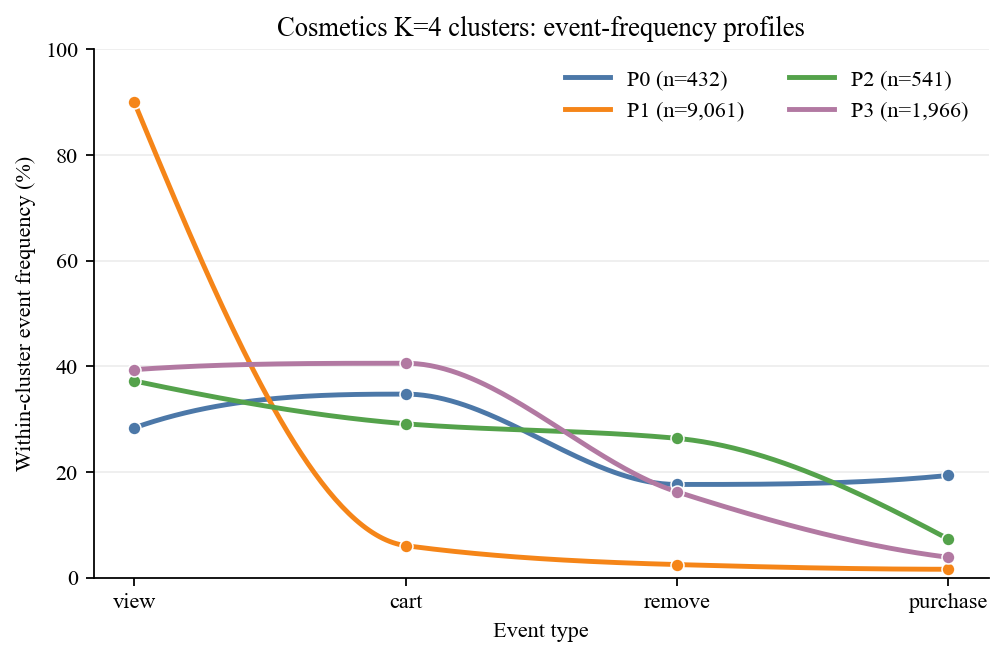
\includegraphics[width=\columnwidth]{img/analysis/cosmetics_k4_event_frequency.png}
\caption{$K=4$ 사용자 임베딩 군집 P0--P3의 군집 내 이벤트 빈도(\%). 점은 관측값이고
곡선은 네 행동 범주 사이를 PCHIP으로 연결한 시각적 보간이다.}
\label{fig:eventmix}
\end{figure}

\subsection{Maximum-entropy 행동과 세션 간격}
세션 내 선택은 \texttt{view}, \texttt{cart}, \texttt{remove}, \texttt{purchase},
\texttt{end}의 다섯 행동이다. 상태에는 세션 위치와 경과시간, 직전 이벤트 간격,
과거 행동 횟수와 직전 행동을 사용한다. 11개 비절편 특징의 선형항, 제곱항 및 모든
2변수 교차항을 포함하여 78차원 특징 $\phi^{(2)}(s)$를 구성한다. 사용자 $u$의
즉시 보상과 선택확률은
\begin{align}
r_u(s,a)&=\theta_{u,a}^{\top}\phi^{(2)}(s),\\
\pi_u(a\mid s)&=\frac{\exp r_u(s,a)}{\sum_{a'}\exp r_u(s,a')}
\end{align}
이다. Temperature는 1로 고정하고 각 특징에서 다섯 행동 계수의 합을 0으로 제약한다.
대표 사용자 계수에는 3성분 대각 GMM을 적합하며, 모집단 혼합비는 P0 14.70\%,
P2 18.41\%, P3 66.89\%로 보정한다. 이는 장기 occupancy를 일치시키는 완전한
trajectory IRL이 아니라 상태조건부 maximum-entropy 선택모형이다~\cite{ziebart2008}.

\noindent\begin{minipage}{\columnwidth}
\vspace{2pt}\hrule\vspace{2pt}
\noindent\textbf{Algorithm 2: Persona-conditioned maximum-entropy IRL}\par
\vspace{2pt}\hrule\vspace{3pt}
\noindent\textbf{Input:} $D$, $\{c_u\}$\par
\noindent\textbf{Output:} $q(\theta)$, $q(\tau\mid s_{\mathrm{end}})$\par
\begin{tabular}{@{}r@{\hspace{0.6em}}l@{}}
1 & $X\leftarrow\phi^{(2)}(D)$\\
2 & \textbf{for each} persona $c$ \textbf{do}\\
3 & \quad $\theta_c\leftarrow\arg\min_\theta
      \mathcal L_{\mathrm{MaxEnt}}(X_c,\theta)$\\
4 & \quad $\theta_u\leftarrow\operatorname{MAP}(D_u\mid\theta_c)$\\
5 & \textbf{end for}\\
6 & $q(\theta)\leftarrow\operatorname{GMM}(\{\theta_u\})$\\
7 & $q(\tau\mid s_{\mathrm{end}})\leftarrow\operatorname{MaxEntGap}(D)$\\
\end{tabular}
\vspace{2pt}\hrule
\end{minipage}

\texttt{end} 이후 간격은 0--1시간, 1--6시간, 6--24시간, 1--3일, 3--7일,
7--14일, 14--30일, \texttt{NO\_RETURN\_30D}의 여덟 토큰으로 샘플링한다. 첫 세션의
직전 간격은 학습 평균 51.33시간으로 초기화하되 결측 여부를 별도 지시자로 유지한다.
내부상태 engagement, friction, satiation, inactivity momentum, gap acceleration,
habit strength는 과거 세션으로 재귀 갱신되어 행동 효용과 복귀 간격을 조절한다.
NEW, home persona, CHURNING 및 두 종료상태의 전이는 그림~\ref{fig:lifecycle}과 같다.

\subsection{합성 uplift 모듈}
\noindent\begin{minipage}{\columnwidth}
\vspace{2pt}\hrule\vspace{2pt}
\noindent\textbf{Algorithm 3: Sequential uplift calibration}\par
\vspace{2pt}\hrule\vspace{3pt}
\noindent\textbf{Input:} $G$, $Z$, $\{\pi_c^{\mathrm{can}},\Delta_c^*\}_{c\in\mathcal C}$\par
\noindent\textbf{Output:} $W^*$, $\lambda^*$\par
\begin{tabular}{@{}r@{\hspace{0.6em}}l@{}}
1 & $G\leftarrow\operatorname{freeze}(G)$\\
2 & $W^*\leftarrow\operatorname{FitCanonical}(Z,\pi^{\mathrm{can}})$\\
3 & \textbf{for each} $k=0,\ldots,K-1$ \textbf{do}\\
4 & \quad $\widehat\Delta^{(k)}\leftarrow
      \operatorname{PairedRollout}(G,W^*,\lambda^{(k)},\omega_k)$\\
5 & \quad $\lambda_c^{(k+1)}\leftarrow\lambda_c^{(k)}
      \Delta_c^*/\widehat\Delta_c^{(k)}$\\
6 & \textbf{end for}\\
7 & $\lambda^*\leftarrow
      \lambda^{(\arg\min_k\|\widehat\Delta^{(k)}-\Delta^*\|_2)}$\\
\end{tabular}
\vspace{2pt}\hrule
\end{minipage}

\begin{figure*}[!t]
\centering
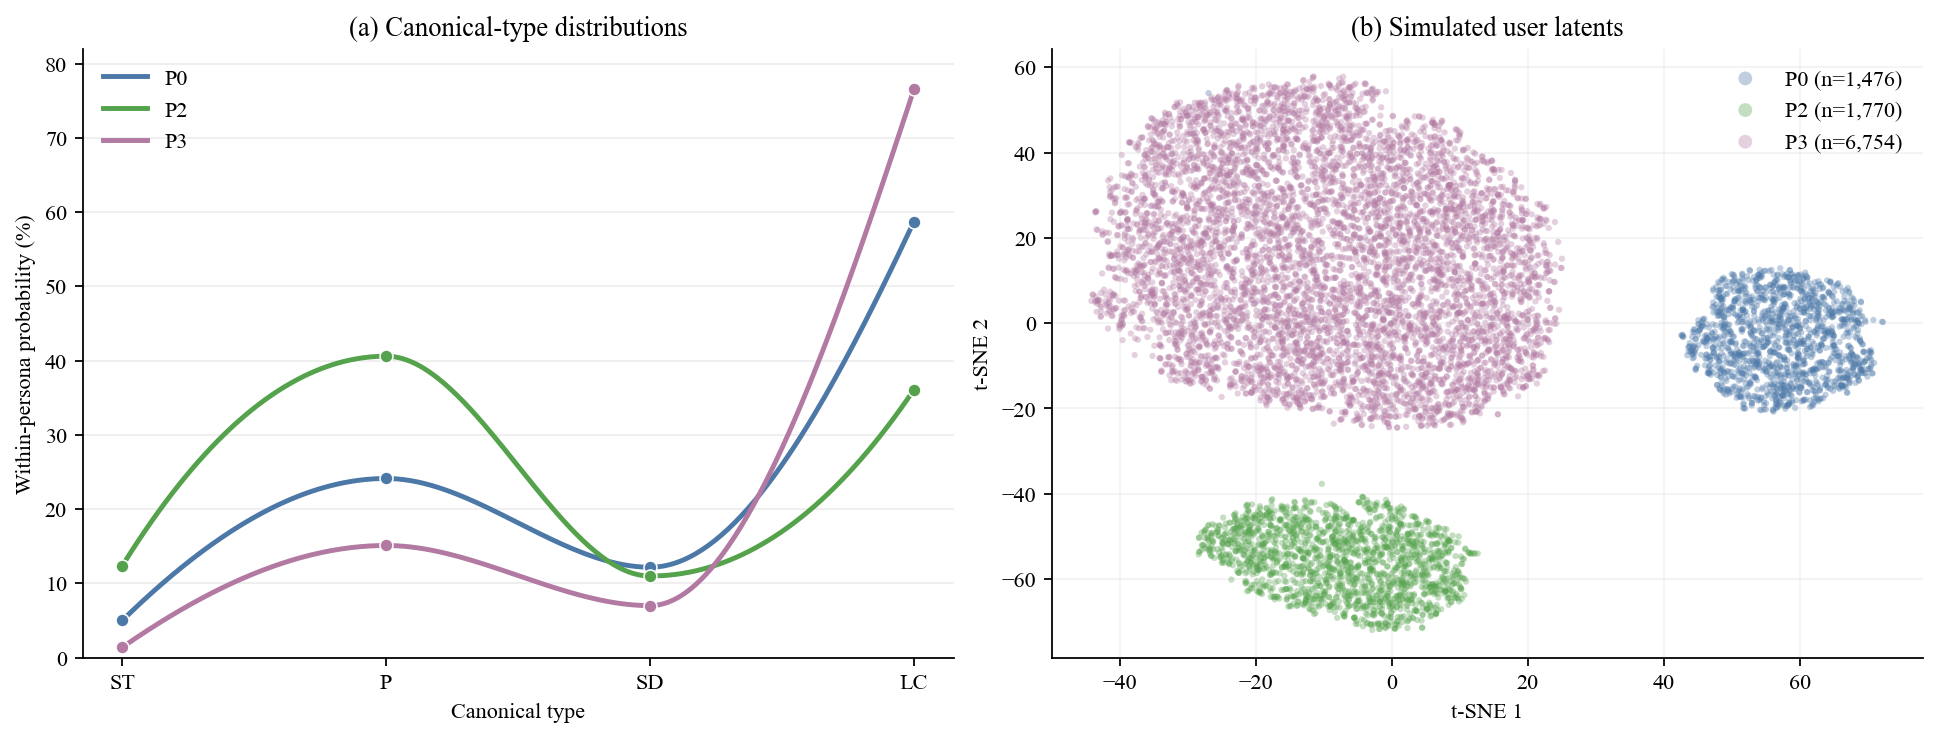
\includegraphics[width=0.64\textwidth]{img/analysis/figure3_simulated_user_distribution.png}
\caption{합성 사용자 분포. (a) 최대엔트로피 결합의 persona별 canonical-type 분포.
ST, P, SD, LC는 sure thing, persuadable, sleeping dog, lost cause다. (b) 합성 사용자
10,000명의 48차원 latent에 대한 t-SNE 투영이며 좌표축은 생성에 사용하지 않는다.}
\label{fig:canonical-latent}
\end{figure*}

Tianchi에는 장바구니와 세션 경계가 없으므로 처치 이전의 공통 행동공간만 사용한다.
사용자 $i$의 행동요약과 대리군, Cosmetics persona 대응은
\begin{equation}
\begin{gathered}
h_i^-=(n_{i,\mathrm{click}}^-,n_{i,\mathrm{purchase}}^-,
n_{i,\mathrm{active}}^-),\qquad
g_i=\Gamma(h_i^-;q_{.25},q_{.75},q_{.95}),\\
m(0)=g_{\mathrm{purchase}},\qquad
m(2)=g_{\mathrm{deep}},\qquad
m(3)=g_{\mathrm{browse}}
\end{gathered}
\end{equation}
로 정의한다. 여기서 $\Gamma$는 처치 이전 활동량과 구매 유무의 분위수 규칙이며,
$m$은 공통된 탐색 깊이와 구매 이력을 이용한 persona--proxy 대응이다. $H=14$,
$A_i\in\{0,1\}$ 및 $Y_i^{(H)}=\mathbb{1}[\sum_{d=1}^{H}N_{i,d}^{\mathrm{purchase}}>0]$에 대해
\begin{equation}
p_{c,a}=\mathbb{E}[Y_i^{(H)}\mid g_i=m(c),A_i=a],\qquad
\Delta_c^*=p_{c,1}-p_{c,0}
\end{equation}
를 보정 모멘트로 둔다. 주변분포를 보존하면서 추가 상관을 주입하지 않는
최대엔트로피 결합을 위해
\begin{equation}
\mathcal T=\{ST:(1,1),\ P:(0,1),\ SD:(1,0),\ LC:(0,0)\}
\end{equation}
의 네 canonical type을 정의한다. 각 순서쌍은 $(Y^{(H)}(0),Y^{(H)}(1))$이며,
각 persona의 목표분포는
\begin{equation}
\begin{aligned}
\pi_{c,ST}&=p_{c,0}p_{c,1}, & \pi_{c,P}&=(1-p_{c,0})p_{c,1},\\
\pi_{c,SD}&=p_{c,0}(1-p_{c,1}), &
\pi_{c,LC}&=(1-p_{c,0})(1-p_{c,1})
\end{aligned}
\end{equation}
48차원 사용자 latent에 절편을 붙인 $49\times4$ 행렬과 softmax로 개인별 canonical
type 확률을 생성하고 persona별 평균이 목표분포를 근사하도록 학습한다.
그림~\ref{fig:canonical-latent}(a)는 persona별 목표분포를 나타낸다.
Persuadable에는 양의 쿠폰 offset, sleeping dog에는 음의
offset, 나머지 두 유형에는 0을 준다. 각 수령효과는
\begin{equation}
d(k)=\left[\max\left(0,1-\frac{\lfloor k/7\rfloor}{5}\right)\right]^2,
\qquad E_t=\sqrt{\sum_{r<t}d(t-r)}
\end{equation}
로 35일 안에 단조 감소하며, 제곱근으로 반복 수령의 한계기여를 줄인다. 쿠폰이 없거나
strength가 0이면 모든 offset이 0이 되어 무쿠폰 생성기를 정확히 복원한다.

본 단계는 행동 생성기를 계속 갱신하는 continual learning이 아니다. Cosmetics에서
학습한 reward, coefficient GMM 및 세션 간격 모형을 동결한 뒤, Tianchi 모멘트를
이용해 canonical-type 매핑과 persona별 쿠폰 강도만 순차적으로 보정한다. 따라서
무쿠폰 행동 적합도를 보존하면서 uplift 가정만 별도로 교체하거나 검증할 수 있다.
\section{실험 결과}
\subsection{사용자 생성기와 uplift 보정}
무쿠폰 10,000명에서 행동비율 RMSE는 0.0540, 구매 세션률은 관측 4.23\% 대비
생성 3.94\%, 30일 비복귀율은 26.24\% 대비 21.91\%였다. 2차 reward는 persona
평균 NLL을 0.648에서 0.600으로, lifecycle 상태는 0.840에서 0.808로 낮췄다.
별도 6,000명으로 보정하고 10,000명으로 검증한 결과
$|\widehat\Delta_{\mathrm{pop}}-\Delta_{\mathrm{pop}}^*|=0.07\%p$였다.
그림~\ref{fig:canonical-latent}(b)는 보정된 home-persona 혼합비에서 생성한 latent의
t-SNE 투영이며, 좌표는 생성이나 분류에 사용하지 않는다.

\begin{figure}[b]
\centering
\resizebox{0.52\columnwidth}{!}{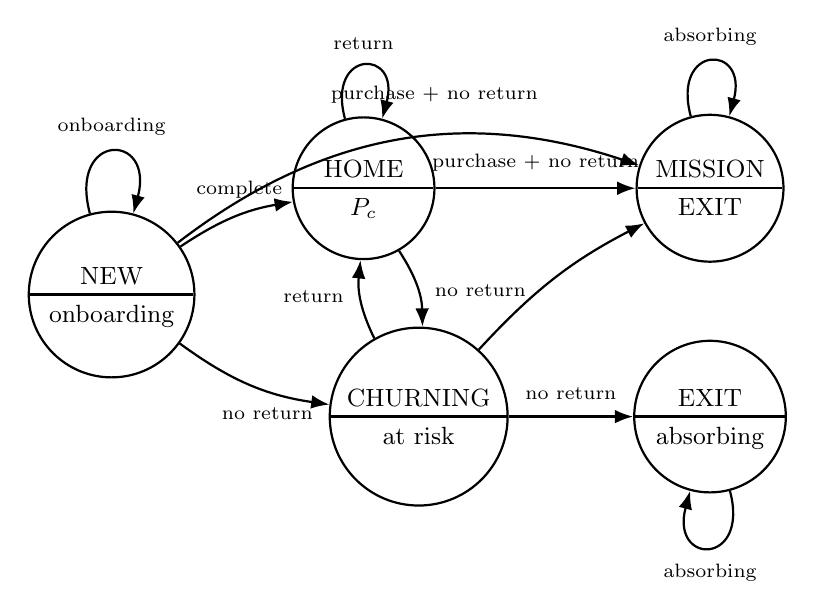
\begin{tikzpicture}[
  >=Latex,
  state/.style={circle split, draw, line width=.8pt, minimum size=18mm,
    align=center, font=\small},
  flow/.style={->, line width=.8pt},
  note/.style={font=\scriptsize, inner sep=0pt}
]
\node[state] (new) at (-4.4,0) {NEW\nodepart{lower}onboarding};
\node[state] (home) at (-1.2,1.35) {HOME\nodepart{lower}$P_c$};
\node[state] (churn) at (-.5,-1.55) {CHURNING\nodepart{lower}at risk};
\node[state] (mission) at (3.2,1.35) {MISSION\nodepart{lower}EXIT};
\node[state] (exit) at (3.2,-1.55) {EXIT\nodepart{lower}absorbing};

\draw[flow] (new) to[loop above, looseness=5] node[note, above=2mm] {onboarding} (new);
\draw[flow] (new) to[bend left=12] node[note, pos=.55, above=2mm] {complete} (home);
\draw[flow] (new) to[bend right=14] node[note, pos=.62, below=2mm] {no return} (churn);
\draw[flow] (new) to[bend left=28] node[note, pos=.58, above=4mm] {purchase + no return} (mission);

\draw[flow] (home) to[loop above, looseness=5] node[note, above=2mm] {return} (home);
\draw[flow] (home) to[bend left=16] node[note, pos=.55, right=2mm] {no return} (churn);
\draw[flow] (churn) to[bend left=16] node[note, pos=.55, left=2mm] {return} (home);
\draw[flow] (home) -- node[note, midway, above=2mm] {purchase + no return} (mission);
\draw[flow] (churn) to[bend left=10] (mission);
\draw[flow] (churn) -- node[note, midway, above=2mm] {no return} (exit);

\draw[flow] (mission) to[loop above, looseness=5] node[note, above=2mm] {absorbing} (mission);
\draw[flow] (exit) to[loop below, looseness=5] node[note, below=2mm] {absorbing} (exit);
\end{tikzpicture}
}
\caption{세션 종료 시 적용되는 lifecycle 전이. $P_c$는 출생 시 고정된 home
persona이고 MISSION EXIT와 EXIT는 30일 비복귀를 나타내는 흡수상태다.}
\label{fig:lifecycle}
\end{figure}

\subsection{주간 쿠폰 정책 비교}
정책은 사용자별 주 1회 쿠폰 발송 여부를 결정하고 이후 7일의 구매, 세션과 쿠폰비를
합산하여 직전 선택의 feedback으로 받는다. 관측 상태는 persona와 lifecycle,
최근 7일 및 30일 행동, 마지막 세션과 구매 이후 경과일, 쿠폰 노출과 발송 가능 여부의
19개 과거정보 특징이다. 목적함수는
\begin{equation}
R=1000N_{\mathrm{purchase}}-100N_{\mathrm{coupon}}
\end{equation}
이다. UCB, TS, LinUCB, LinTS, PPO~\cite{schulman2017}, discrete SAC~\cite{haarnoja2018}를
1,000명, 13주 동안 학습하고 별도 5,000명, 52주에서 고정 정책을 평가하였다.

\begin{table}[t]
\centering
\caption{주간 쿠폰 정책의 1년 고정 정책 평가: 평균(표준편차)}
\label{tab:policy}
\small
\setlength{\tabcolsep}{2pt}
\begin{tabular*}{\columnwidth}{@{\extracolsep{\fill}}lrrr@{}}
\toprule
Policy & Profit/user ($\times10^3$) & Purch./user & Coupons/user\\
\midrule
UCB & 27.69 (75.21) & 32.89 (75.21) & 52.00 (0.00)\\
TS & 27.69 (75.21) & 32.89 (75.21) & 52.00 (0.00)\\
LinUCB & 28.96 (73.15) & 30.76 (74.35) & 18.01 (18.76)\\
LinTS & 29.40 (73.34) & 31.36 (74.51) & 19.63 (19.20)\\
PPO & 27.69 (75.21) & 32.89 (75.21) & 52.00 (0.00)\\
\textbf{Discrete SAC} & \textbf{30.89 (73.83)} & \textbf{32.98 (75.07)} & \textbf{20.90 (17.00)}\\
Never coupon & 3.35 (2.48) & 3.35 (2.48) & 0.00 (0.00)\\
Weekly coupon & 27.69 (75.21) & 32.89 (75.21) & 52.00 (0.00)\\
\bottomrule
\end{tabular*}
\end{table}

SAC는 매주 발송보다 순이익이 11.56\% 높고 쿠폰은 59.81\% 적게 사용하였다.
PPO는 최종적으로 매주 발송과 같은 정책을 선택했으며 학습기간 oracle 대비 비용이
2,264,500으로 가장 컸다. 본 환경은 약 13,000개의 주간 transition만 제공하므로
on-policy PPO보다 replay를 사용하는 SAC에 표본효율 측면에서 유리할 수 있다.

\section{논의 및 결론}
본 연구는 Cosmetics 기반 행동 생성기와 Tianchi 기반 합성 uplift 모듈을 분리해
순차 쿠폰 정책을 평가하였다. 모듈 분리는 0효과, 감쇠율 및 canonical 결합을 바꾼
민감도 분석을 가능하게 한다.

페르소나는 기술적 군집이고 Tianchi 수령은 비무작위이므로 canonical 분포와 coupon
offset은 인과 추정치가 아니다. 정책 순위 역시 단일 seed와 실험용 비용에 조건부다.
향후 다중 seed, 비용·감쇠 민감도 및 무작위 처치자료 검증이 필요하다.

\begingroup
\small
\setlength{\parindent}{0pt}
\begin{thebibliography}{20}
\bibitem{rees46} REES46, ``Free datasets with eCommerce behavior data,'' \url{https://rees46.com/en/datasets}.
\bibitem{tianchi} Alibaba Cloud Tianchi, ``O2O Coupon Usage Prediction Dataset,'' \url{https://tianchi.aliyun.com/dataset/5903}.
\bibitem{sun2019} F. Sun et al., ``BERT4Rec: Sequential Recommendation with Bidirectional Encoder Representations from Transformer,'' \textit{CIKM}, 2019.
\bibitem{cho2014} K. Cho et al., ``Learning Phrase Representations using RNN Encoder-Decoder for Statistical Machine Translation,'' \textit{EMNLP}, 2014.
\bibitem{ziebart2008} B. D. Ziebart et al., ``Maximum Entropy Inverse Reinforcement Learning,'' \textit{AAAI}, 2008.
\bibitem{devriendt2018} F. Devriendt, D. Moldovan, and W. Verbeke, ``A Literature Survey and Experimental Evaluation of the State-of-the-Art in Uplift Modeling,'' \textit{Big Data}, 6(1), 2018.
\bibitem{ie2019} E. Ie et al., ``RecSim: A Configurable Simulation Platform for Recommender Systems,'' arXiv:1909.04847, 2019.
\bibitem{rohde2018} D. Rohde et al., ``RecoGym: A Reinforcement Learning Environment for Product Recommendation in Online Advertising,'' arXiv:1808.00720, 2018.
\bibitem{shi2019} J.-C. Shi et al., ``Virtual-Taobao: Virtualizing Real-World Online Retail Environment for Reinforcement Learning,'' \textit{AAAI}, 2019.
\bibitem{li2010} L. Li et al., ``A Contextual-Bandit Approach to Personalized News Article Recommendation,'' \textit{WWW}, 2010.
\bibitem{agrawal2013} S. Agrawal and N. Goyal, ``Thompson Sampling for Contextual Bandits with Linear Payoffs,'' \textit{ICML}, 2013.
\bibitem{schulman2017} J. Schulman et al., ``Proximal Policy Optimization Algorithms,'' arXiv:1707.06347, 2017.
\bibitem{haarnoja2018} T. Haarnoja et al., ``Soft Actor-Critic: Off-Policy Maximum Entropy Deep Reinforcement Learning with a Stochastic Actor,'' \textit{ICML}, 2018.
\end{thebibliography}
\endgroup

\end{document}
